\documentclass[resume]{subfiles}



\begin{document}
\section{XF et Machines d'états}
\begin{enumerate}
\item États
\begin{enumerate}
\item Action sur entrée
\item Action continue
\item Action sur sortie
\end{enumerate}
\item Transistions
\begin{enumerate}
\item déclenchée par un événement
\item Condition
\item Action
\end{enumerate}
\end{enumerate}
\begin{figure}[H]
\centering
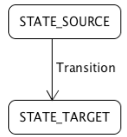
\includegraphics[width=2.00cm]{img_8.png}
\end{figure}
\begin{figure}[H]
\centering
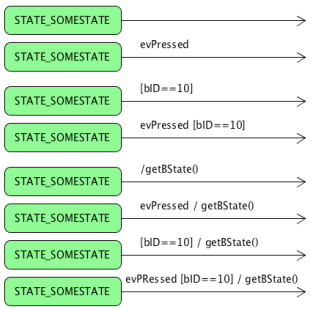
\includegraphics[width=4.00cm]{img_9.png}
\end{figure}
\subsection{XF}
Atomique : Pas d'interruptions
\end{document}